\documentclass[a4paper,12pt,titlepage]{article}
\usepackage[portuguese]{babel}
\usepackage[utf8]{inputenc}
\usepackage[T1]{fontenc}
\usepackage{mathtools}
\usepackage{amssymb}
\usepackage{amsmath}
\usepackage{algorithm}% http://ctan.org/pkg/algorithms
\usepackage{algpseudocode}% http://ctan.org/pkg/algorithmicx
\usepackage{url}
\usepackage{texdraw}
\usepackage{gnuplottex}
\usepackage{caption}
\usepackage{subcaption}
\usepackage[section]{placeins}
\usepackage{booktabs}
\let\biconditional\leftrightarrow
\begin{document}

\title{Relatório do Trabalho de Conceção e Análise de Algoritmos}
\date{27 de abril 2015}
\author{Francisco Veiga, up201201604@fe.up.pt
 \and João Cabral, up201304395@fe.up.pt
 \and  João Mota, up201303462@fe.up.pt\linebreak
 \and Faculdade de Engenharia da Universidade do Porto}
%\input{./title_page_1.tex}
\maketitle
\tableofcontents
\listoffigures
\listoftables
\newpage
\section{Introdução}

No contexto da unidade curricular de Conceção e Análise de Algoritmos, foi solicitada a conceção de um programa de compressão de ficheiros.

\section{Problemas a abordar} 
Para o presente trabalho foi pedida a conceção de um programa de compressão, de seu nome `LeZip', que se baseia em três algoritmos: \emph{Algoritmo de Huffman}, \emph{Algoritmo de Lempel-Ziv-Welch} e \emph{Run Length Encoding}.


\section{Casos de Utilização}
Está implementada a funcionalidade que permite ao utilizador passar uma pasta ao programa e escolher o algoritmo de compressão desejado. O programa irá prontamente gerar uma pasta semelhante com os ficheiros comprimidos. O mesmo programa poderá também executar a operação inversa, gerando uma pasta semelhante à primeira.

\newpage
\section{Formalização do problema}

\subsection{Algoritmo de Huffman}

\subsubsection*{Inputs}
\begin{itemize}
\item{Um alfabeto $A = \{a_1, a_2, ... , a_n\}$ de carateres presentes no ficheiro a comprimir.}
\item{Uma lista de frequências $F = \{f_1, f_2, ..., f_n\}$ onde $f_i = peso(a_i), 1 \leq i \leq n$ .}
\end{itemize}

\subsubsection*{Outputs}
\begin{itemize}
\item{Uma lista de códigos binários $C(A,F) = \{c_1, c_2, ..., c_n\}$ onde $c_i$ é o código de $a_i, 1 \leq i \leq n$ e $|c_i|$ é o comprimento em bits de $c_i$.}
\end{itemize}

\subsubsection*{Função Objetivo}
Seja $L(C)=\displaystyle\sum_{i=1}^{n}f_i |c_i|$. Pretende-se encontrar $C(A,F)$ que minimize $L(C)$.
\subsection{Algoritmo LZW}
\subsubsection*{Inputs}
\begin{itemize}
\item{Um dicionário de símbolos $D = \{d_1, d_2, ..., d_n\}$}
\item{Uma mensagem $M=\{m_1, m_2, ..., m_l\}$ tal que $\forall m \in M (\exists d \in D(m = d))$}
\end{itemize}
\subsubsection*{Outputs}
\begin{itemize}
\item{O dicionário $D$ acrescido de algumas combinações de símbolos consecutivos de $M$.}
\end{itemize}
\newpage
\section{Considerações sobre \emph{Run Length Encoding}}
Não é feita uma análise formal do algoritmo de Run Length Encoding. Sobre o mesmo é portanto elaborada a seguinte explicação.\newline
O RLE é uma técnica de compressão, que permite comprimir cadeias de caracteres onde existam sequencias longas de caracteres repetidos.\newline
O principio deste algoritmo é simples, quando temos a ocorrência de uma repetição continuada de um carácter, por exemplo, BBBBBBB é possível representá-lo da seguinte forma 7B. No entanto não podemos simplesmente substituir no meio de um texto a sequência de caracteres por números porque iria ser extremamente difícil detetar situações em que fossem usados algarismos no texto.\newline
Neste caso temos que distinguir se o algarismo já estava presente no texto ou se foi introduzido pela codificação. Assim se usarmos por exemplo um carácter especial podemos identificar o início da codificação por exemplo *7B. \newline
Esta técnica só é eficiente se a sequência tiver um tamanho maior de 3, além disso o carácter especial não pode ser um dos caracteres que ocorrem no texto.
\subsection{Compressão de textos}
Para a compressão de textos este método não é muito eficiente. Por exemplo, na Europa não é muito comum as repetições de três ou mais  letras. Repetições de 4 caracteres iguais só ocorreriam em tabelas, quadros, ou com caracteres especiais (final de linha, espaços, tabulações, etc).
\subsection{Compressão de imagens}
Na compressão de imagens esta técnica é mais promissora pois imagens apresentam maiores áreas continuas da mesma cor.
\subsection{Codificação}
Admita-se a seguinte mensagem a codificar:AAAAAAACVBDDDDDDDDDD\newline
Este algoritmo recebe um ficheiro de texto com sequências de carateres, lê-os um a um, e na eventualidade de haver repetição continuada de um carácter é aplicado o algoritmo, caso contrário o mesmo é escrito.
\newline
No exemplo em questão o resultado seria 7ACVB*10D.
\subsection{Descodificação}
Admita-se a seguinte mensagem a descodificar:*7ACVB*10D\newline
Este algoritmo recebe um ficheiro comprimido, lê carácter a carácter,e caso encontre o carácter especial lê o carácter a seguir, que é o numero de caracteres a escrever do carácter a seguir, se não escreve o carácter.\newline
No exemplo em questão o resultado seria AAAAAAACVBDDDDDDDDDD.
\newpage
\section{Algoritmos Implementados}
\subsection{Huffman}
\begin{algorithmic}
\Procedure{HUFFMAN-TREE}{$f :[f_1, f_2, ..., f_n], f_i=w(i)$}
\State $T \gets \text{Árvore Binária vazia}$
\State $Q \gets \text{Fila de prioridade iniciada com os nós da lista }f$
\For {$k=1$ to $k = n-1$}
\State $left \gets \text{EXTRACT-MIN(Q)}$
\State $right \gets \text{EXTRACT-MIN(Q)}$
\State $node \gets \text{CREATE-NODE(T, left, right)}$
\State $\text{INSERT-NODE(T, left, right)}$
\State $\text{INSERT-QUEUE(node)}$
\EndFor\newline
\Return $T$
\EndProcedure
\Procedure{HUFFMAN-ENCODE\footnote{O procedimento para descodificar é análogo}}{in, out, T : HuffmanTree}
\For{$character \in in$}
\State $out \gets \text{FIND(T,character)}$
\EndFor
\EndProcedure
\end{algorithmic}
\newpage
\subsection{LZW}
\begin{algorithmic}
\Procedure{LZW-ENCODE}{inputstream, outputstream}
\State $d \gets \text{INITIALIZE-DICTIONARY}$
\State $curr \gets 0$
\State $next \gets 1$
\State $s \gets inputstream$
\While{$curr < s.size}$
\State $currString \gets \text{SUBSTRING(s, curr, next)}$
\While{$currString \in d$}
\State $next \gets next+1$
\State $currString \gets \text{SUBSTRING(s, curr, next)}$
\EndWhile
\State $output \gets \text{substring(s, curr, next-1)}$
\State $outputstream \gets output$
\State $\text{INSERT(d, currString)}$
\State $curr \gets next-1$
\State $next \gets curr+1$
\EndWhile
\EndProcedure

\Procedure{LZW-DECODE}{instream, outstream}
\State $d \gets \text{INITIALIZE-DICTIONARY}$
\State $bits \gets outstream$
\State $s \gets ""$
\State $temp \gets ""$
\While{$|bits| \neq 0$}
\State $NumberOfBits \gets \text{CEILING(log2(|d|))}$
\State $code \gets \text{NEXT-CODE(bits)}$
\If{$code \in d$}
\State $temp \gets s$
\State $s \gets \text{FIND(d, code)}$
\State $newEntry \gets tempo$
\Else
\State $newEntry \gets s$
\EndIf
\State $newEntry \gets \text{CONCATENATE(newEntry, SUBSTRING(s, 0, 1))}$
\State $\text{INSERT(d, newEntry)}$
\State $outstream \gets s$
\EndWhile
\EndProcedure
\end{algorithmic}

\section{Análise de Complexidade}\label{Análise de Complexidade}
\subsection{Huffman Tree}
Seja \emph{n} o número de símbolos de uma mensagem sobre um alfabeto de dimensão \emph{m}.
É necessário percorrer duas vezes a mensagem, uma para contar as frequências de cada símbolo e outra para codificar a mensagem. Para construir a árvore de Huffman propriamente dita é necessário inserir cada símbolo do alfabeto na fila de prioridade, o que e uma operação realizável em tempo logarítmico. Temos portanto que a construção da árvore tem uma complexidade $O(mlog(m))$ Acresce a necessidade de percorrer toda a mensagem a codificar e procurar o seu código na árvore binária, o que no caso médio é uma operação $O(log(m))$\footnote{As árvores de Huffman são por natureza árvores desequilibradas. No pior caso a complexidade da operação pode portanto aproximar-se de $O(n)$, para uma árvore degenerada cujo comportamento se assemelha na prática ao de uma lista ligada.}. Repetindo a operação para todos os carateres da mensagem $O(nlog(m))$. Obtém-se portanto uma complexidade $O( (m+n)log(m))$. O valor de $m$ é limitado superiormente pelos 8 bits usados na representação de símbolos, pelo que a sua inclusão na análise assimptótica é de interesse questionável. Na prática o tempo de execução é superiormente limitado pelo tamanho da mensagem, para qualquer mensagem cuja dimensão justifique o overhead associado ao uso de uma Huffman Tree.
\subsection{LZW}
Seja \emph{n} o número de símbolos da mensagem.
O algoritmo percorre a mensagem a codificar uma vez. Para cada símbolo o algoritmo efetua uma inserção num dicionário implementado como uma \emph{Árvore Vermelho-Preto}. Esta operação tem uma complexidade logarítmica pelo que o Algoritmo tem complexidade de codificação $O(nlog(n))$. Para descodificar uma mensagem o processo é análogo, sendo necessário fazer uma procura na dicionário, cuja complexidade é também logarítmica. Obtém-se portanto um tempo semelhante $O(nlog(n))$.
\newpage
\section{Análise Empírica}
\subsection{Taxas de compressão}
\begin{table}[h]
\resizebox{\textwidth}{!}{%
\begin{tabular}{@{}lccccc@{}}
\toprule
\multicolumn{6}{c}{Taxas de compressão dos algoritmos implementados} \\ \midrule
          & \multicolumn{5}{c}{Tipo de ficheiro utilizado}           \\ \cmidrule(l){2-6} 
          & PDF      & Imagem   & Executável  & Texto    & Som       \\ \cmidrule(l){2-6} 
Huffman   & 87.76\%  & 55.30\%  & 117.18\%    & 72.30\%  & 118.08\%  \\ \cmidrule(l){2-6} 
LZW       & 48.32\%  & 36.65\%  & 116.71\%    & 43.37\%  & 117.67\%  \\ \bottomrule
\end{tabular}
}
\caption{Compressão obtida por cada algoritmo implementado sobre diferentes tipos de ficheiros}
\label{my-label}
\end{table}
\newpage
\subsection{Tempo de execução}
Para efetuar uma análisem empírica do tempo de execução de cada programa foram gerados ficheiros aleatórios com tamanhos progressivamente maiores e medidos os respetivos tempos de execução. Os resultados obtidos foram representados sob a forma dos gráficos das figuras \ref{f:1} e \ref{f:2}.
\begin{figure}
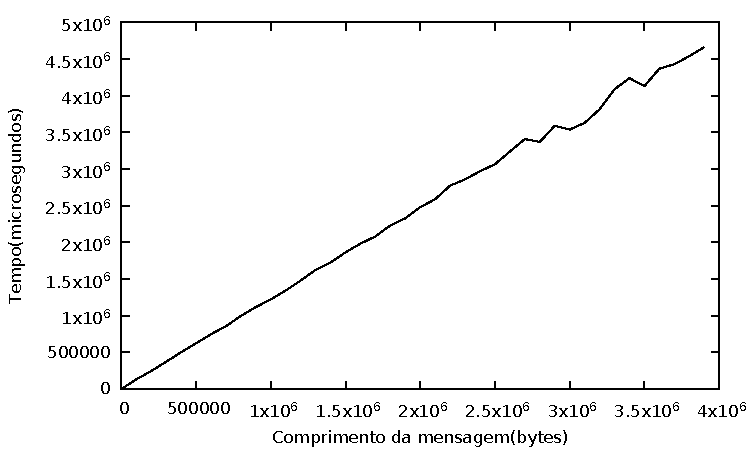
\includegraphics{huff.pdf}
\caption{Variação da performance do algoritmo de compressão usando codificação de Huffman em função do tamanho da mensagem a codificar.}
\label{f:1}
\end{figure}
\begin{figure}
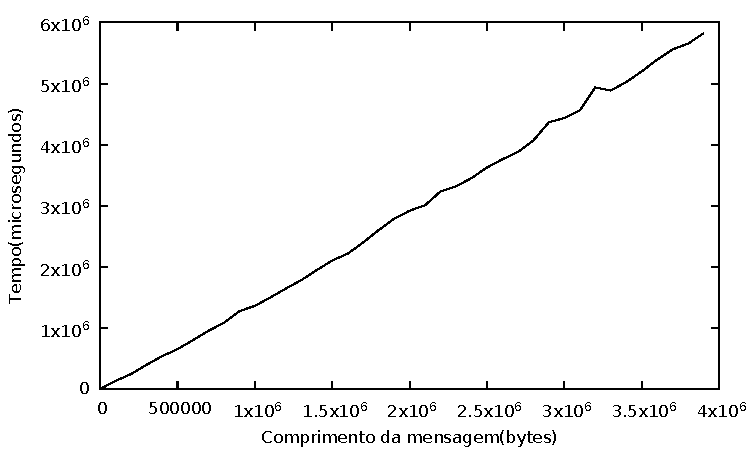
\includegraphics{lzw.pdf}
\caption{Variação da performance do algoritmo de compressão usando LZW em função do tamanho da mensagem a codificar.}
\label{f:2}
\end{figure}
Os resultados da análise empírica parecem confirmar os resultados obtidos na análise teórica efetuada na secção \ref{Análise de Complexidade} da página \pageref{Análise de Complexidade}, aumentando de forma \emph{quasilinear} com o tamanho da mensagem a codificar.
\end{document}
